\subsubsection{University of Virginia} 
%
\paragraph*{Large EIC GEM prototype with 2D U-V strip readout}%\mbox{}\\
\subparagraph*{\textbf  Characterization with Cosmics:}
% 
\begin{figure}[htb]
\centering
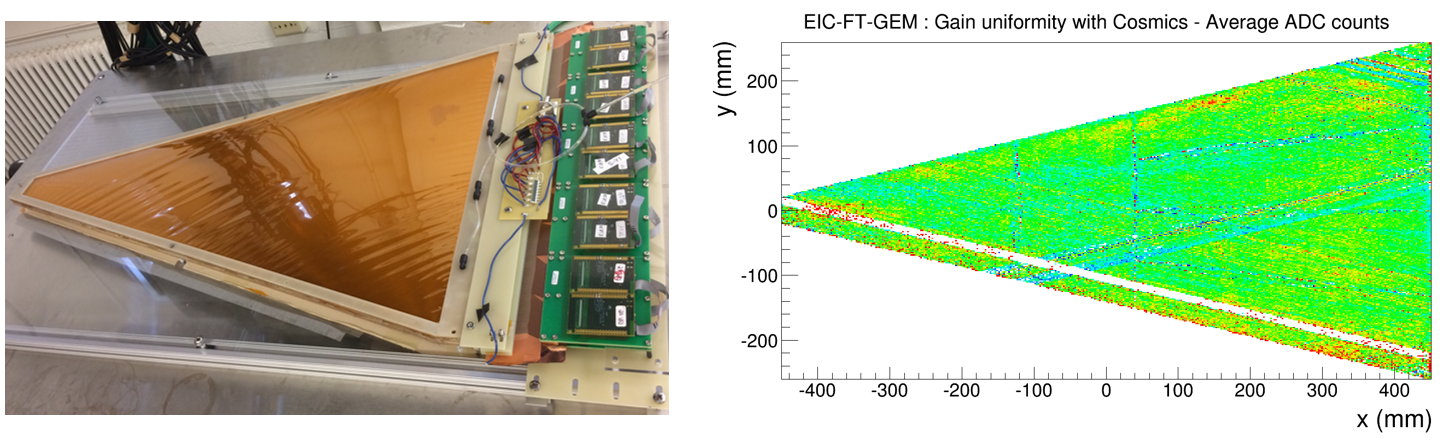
\includegraphics[width=1\columnwidth,trim={0pt 0mm 0pt 0mm},clip]{UVa_plots/eicCosmics}
\caption{\label{fig:eicCosmics}({\it Left:}) UVa large GEM prototype on the cosmic bench at UVa;  ({\it right:}) Gain uniformity: Distribution of the average charge in ADC counts.}
\end{figure}
%
Preliminary tests of the large EIC GEM prototype with cosmics showed a detector gain about an order of magnitude lower than the expected gain of ~8000 of a typical triple-GEM operating with Ar-CO2 (70/30) mixture at the nominal voltage 4.1kV. A likely explanation of the lower gain can be a explained by GEM hole geometry from the production batch for our foil, slightly different from  bi-conical (70-50-70 $\mu$m) shape  of the holes of standard GEM foils. In this case, even a relatively modest gain drop per GEM foil results to a significant gain drop in a triple-GEM detector configuration. Increasing the voltage on the divider from 4.1kV to 4.3kV was enough to restore the nominal operating gain. However, due the large detector size and various challenges related to the  stretching of the GEM foils during the assembly, we could not operate the detector in a stable way at 4.3kV. We therefore decided to test the prototype with Ar-CO2 (80/20) mixture instead of Ar-CO2 (70/30) which allow us to operate at a gain of $\sim 10^4$  at 4.1kV. The prototype was then characterized with cosmics for a three weeks period during which we collected 4  million triggered cosmic events. Fig.~\ref{fig:eicCosmics} ({\it top left}) shows the detector on the cosmic stand in the Detector Lab at UVa.  The plot on {\it top right}, shows a fairly uniform distribution of the average ADC (ratio of the total accumulated charge over the number of hits per unit area)  across  the entire active area for 4 millions cosmic events. This is gain uniformity performance of the chamber. The efficiency drop caused by the presence of GEM support spacers can clearly be seen as well as dead area due to a few broken strips.  The overall uniform gain distribution successfully demonstrates that the novel double-sided zebra connection system that we developed for the readout electronics works perfectly as expected. Analysis of the cosmic data is ongoing.
%
\subparagraph*{\textbf Characterization of UVa large GEM prototype in test beam at FNAL:}
%
\begin{figure}[htb]
\centering
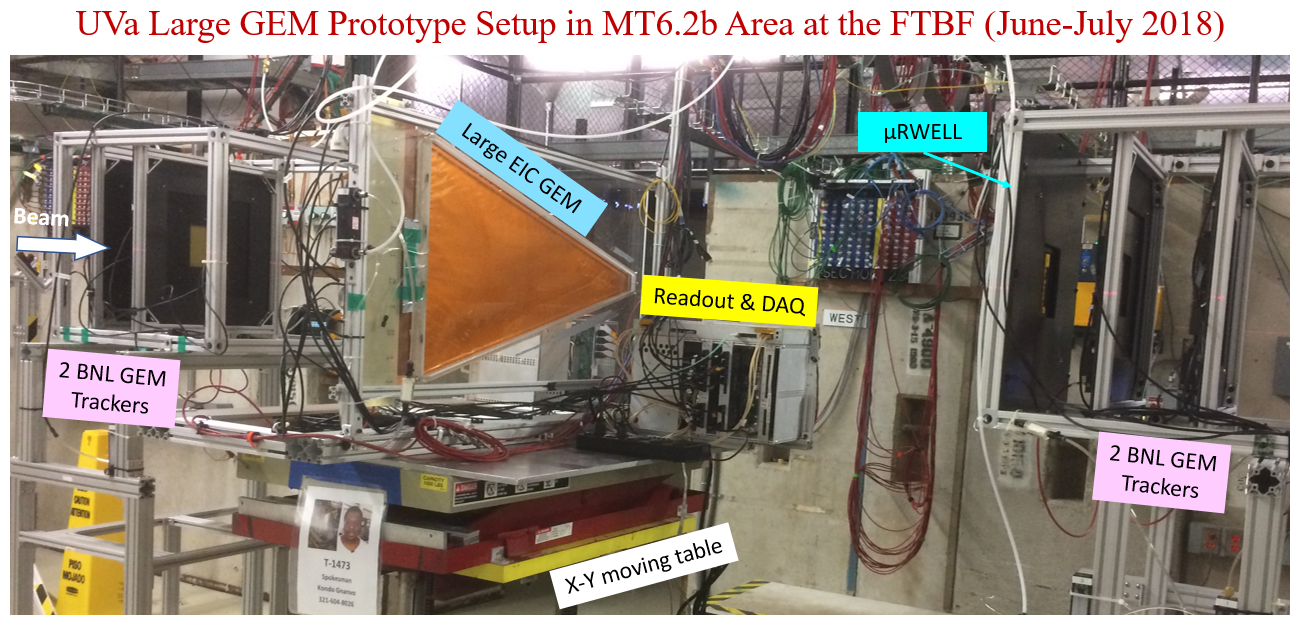
\includegraphics[width=1\columnwidth,trim={0pt 0mm 0pt 0mm},clip]{UVa_plots/ftbfSetup}
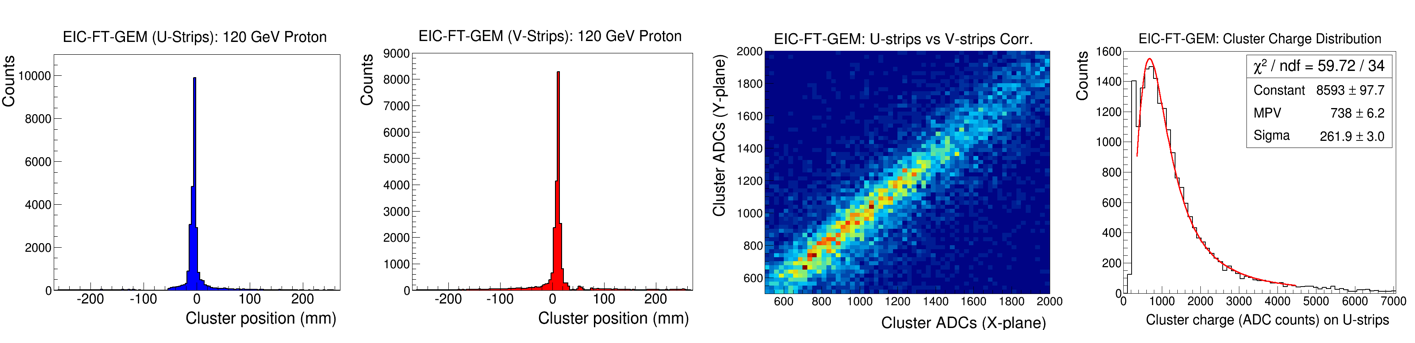
\includegraphics[width=1\columnwidth,trim={0pt 0mm 0pt 0mm},clip]{UVa_plots/eicProtonBeam}
\caption{\label{fig:eicProtonBeam} \textit{Top:} Large GEM setup at FNAL FTBF with two BNL GEMs for the upstream telescope and two other and the  small $\mu$RWELL prototype for the downstream telescope. \textit{Bottom:} Characteristics of the prototype; \textit{Left to right:} 120 GeV proton beam profile on U-strips and V-strips; Charge sharing correlation between the top (U-strips) and bottom (V-strips); Charge distribution in ADC counts on U-strips.}
\end{figure}
%
The large EIC GEM prototype, together with the small $\mu$RWELL prototype and an additional small triple-GEM with 2D zigzag strip prototypes were brought to the Fermilab Test Beam Facility (FTBF) this summer (June 2018 - July 2018) and tested with the 120 GeV primary proton beam  for a period of 3 weeks.
% The beam test campaign was a combined effort which includes M. Hohlmann's group  from Florida Tech (FIT), also testing  their large EIC GEM prototype with zigzag strip readout and K. Dehmelt and T. Hemmick's group from Stony Brook (SBU) testing their small TPC prototype with GEM readout. UVa and FIT shared the same large EIC GEMs setup with the prototypes installed on the X-Y moving table of the  MT6.2b area at the FTBF.
For the tracking, our colleagues from BNL group provided four small triple-GEMs COMPASS readout. The setup is shown on Fig.~\ref{fig:eicProtonBeam} with  BNL GEM trackers and the $\mu$RWELL prototype used as upstream and downstream telescopes. The detector configuration in the setup  was optimized to minimize the  multiple scattering impact on the resolution studies of the EIC GEM prototype. All chambers, including the four BNL GEM trackers operated with the same Ar-CO2 (70/30) gas mixture and the APV25-based Scalable Readout System (SRS) electronics developed at CERN by the RD51 collaboration were used to read out all chambers channels at a trigger rate of $\sim$ 400Hz with the trigger signal from the facility scintillators/PMTs. DATE and AMORE, developed by the CERN ALICE experiment, where used respectively as DAQ software and online/offline  analysis tool.\\
 The plots on the left of Fig.~\ref{fig:eicProtonBeam} show the 120 GeV proton beam profile reconstructed respectively on the top (U-strips) and bottom layers (V-strips) of the U-V readout foil.  Plot on center right shows the excellent correlation of the charges (in ADC counts)  shared between U-strips and V-strips. The  charge distribution (in ADC counts) of the top layer (U-strips) is shown on the right plot. The distribution fits nicely with the Landau function as expected from minimum ionizing particles. This new U-V strips readout foil design developed for this prototype is a clear improvement of the previous iteration that was tested in our  first large EIC GEM prototype in 2013 \cite{Gnanvo:2015xda}. 
%
\subparagraph*{\textbf Issues with the U-V strips readout quality:}
%
\begin{figure}[htb]
\centering
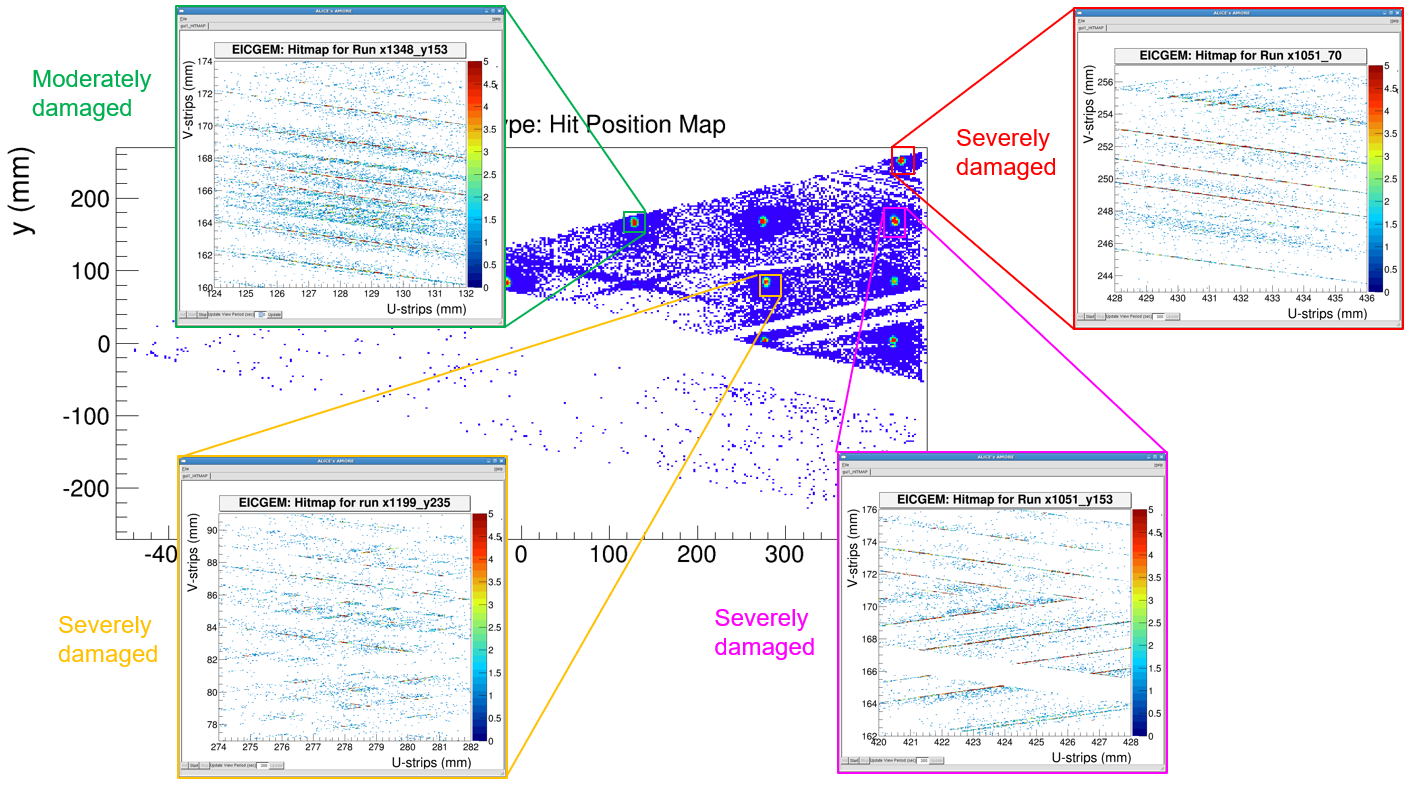
\includegraphics[width=1\columnwidth,trim={0pt 0mm 0pt 0mm},clip]{UVa_plots/eicPosScan}
\caption{\label{fig:eicPosScan}  2D  reconstruction of 120 GeV proton beam from position scan in the top half of the EIC GEM prototype. A zoom in of  reconstructed particle positions for at four beam spots showing some unexpected patterns of non uniform distribution of the reconstructed particle positions likely due to poor production quality of the readout strip layer.}
\end{figure}
%
Fig.~\ref{fig:eicPosScan} shows the 2D reconstruction of the proton beam from a position scan run. A detailed analysis with a fine histogram binning of the area around the beam spot reveals some unexpected patterns of reconstructed positions as can be seen on the four "zoom-in" locations on Fig.~\ref{fig:eicPosScan}. Instead of a uniform distribution of the reconstructed points, what we actually observed  is a picture of  the reconstructed positions heavily concentrated along a set of lines parallel to the strips. As indicated on the plots, the pattern of the reconstructed positions are more pronounced \textit{\textbf{``severe distorsions''}} in some locations than other \textit{\textbf{``moderate distorsions''}} but seems to be present anywhere where we were able to collect data from. These patterns suggests that a significant number of the strips could be shorted both on top and bottom strip layers. A few consecutive shorted strips will destroy the advantage of using  the center of gravity method  to reconstruct the position with high precision and results in the positions reconstructed at the physical center of a single strip and the pattern of highly concentrated parallel lines that we observe in the plots. We are not however completely discarded the possibility that some issues inherent to the zebra strips technology we are using to interface the readout strips to the FE electronics might be the source of distorted signal at the input of the FE readout channels and degrades the position information. We are investigating the  problem with ongoing tests and analysis.
%
\subparagraph*{\textbf Position residual distribution:}
%
\begin{figure}[htb]
\centering
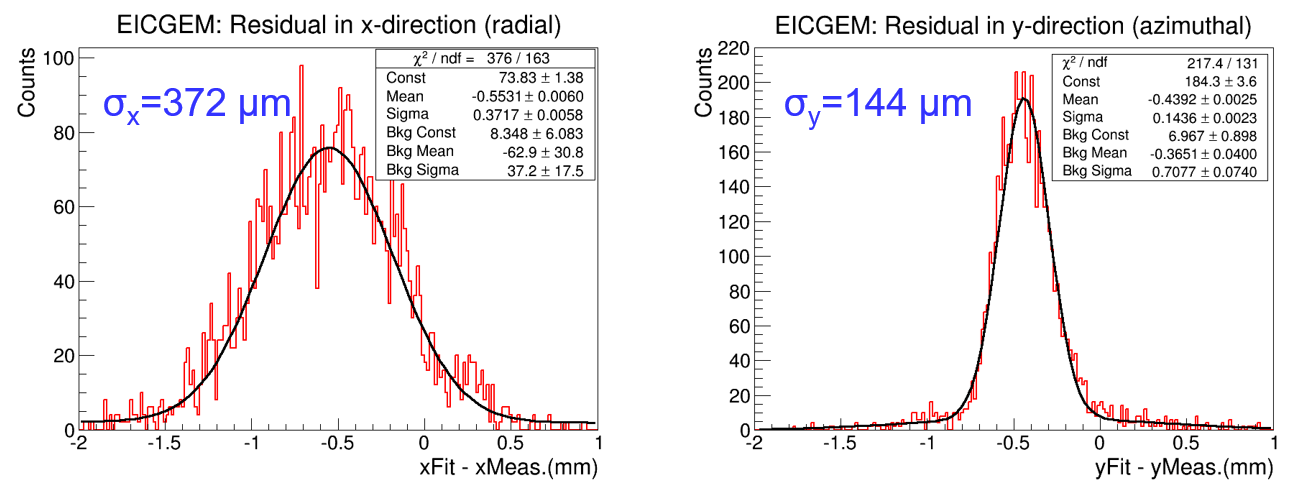
\includegraphics[width=1\columnwidth,trim={0pt 0mm 0pt 0mm},clip]{UVa_plots/eicResidual}
\caption{\label{fig:eicResidual} Residual distribution in x {\it(left:)} and y {\it (right:)} from the proton beam at two locations on the large GEM prototype:  moderate strip distortions area {\it (top plots)} and  severe strip distortions area {\it (bottom plots)} on the large GEM prototype.}
\end{figure}
%
\paragraph*{$\mu$RWELL  prototype with 2D X-Y strip readout}\mbox{}\\
\subparagraph*{\textbf Characterization with Cosmics:}
%
\begin{figure}[htb]
\centering
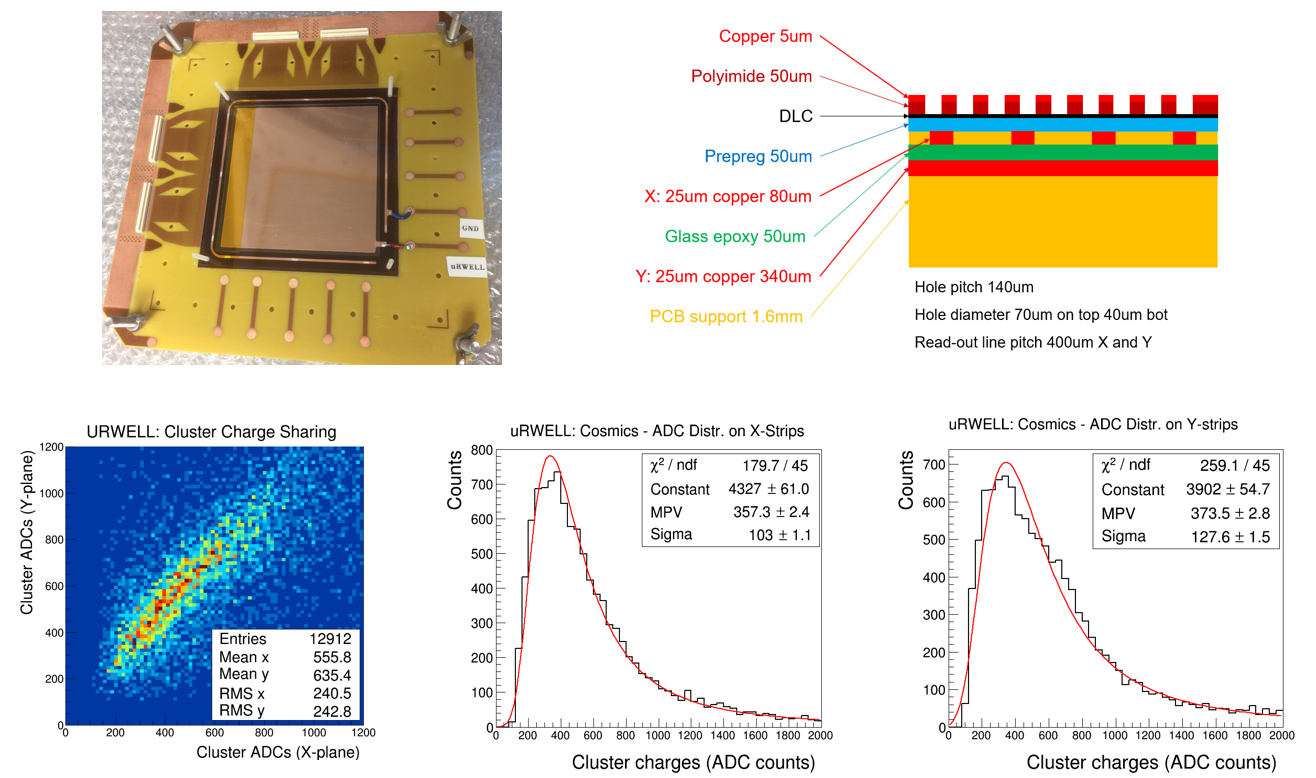
\includegraphics[width=1\columnwidth,trim={0pt 0mm 0pt 0mm},clip]{UVa_plots/uRwellCosmics}
\caption{\label{fig:uRwellCosmics} The $\mu$RWELL prototype with 2D X-Y readout strip, the cross section of the detector is shown at the bottom}
\end{figure}
%
For this Triple-GEM prototype, we use only foils including for the drift cathode and the U-V strips readout board, with no rigid PCB or support structure  in the active area. The 2D U-V strips readout layer and the drift cathode were all produced at CERN from the same copper clad Kapton base material used for the production of GEM foils.The elimination of rigid support structure in the active area of the detector is motivated by for low material requirement to minimize multiple scattering as well as photon induced background. Entrance and exit gas volume with 25 $\mu$m thick Kapton foil have been added to the stack of active foils for pressure balance inside the chamber in order to maintain uniform gap between different layers needed for an uniform gain across the active area.  Top left picture of shows a cross section of the all foils EIC-FT-GEM prototype with the entrance and exit gas windows.
%
\subparagraph*{\textbf FNAL Test Beam results:}
%
\begin{figure}[htb]
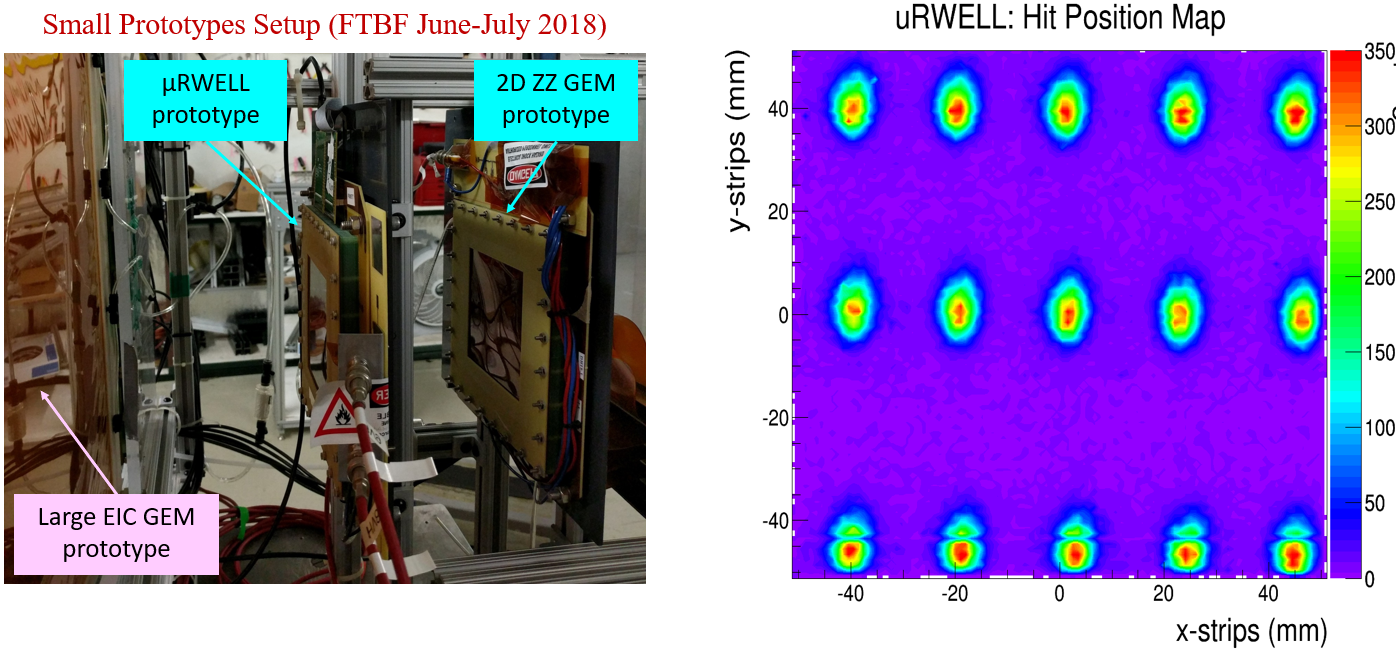
\includegraphics[width=1\columnwidth,trim={0pt 0mm 0pt 0mm},clip]{UVa_plots/ftbfSmallSetup}
\caption{\label{fig:ftbfSmallSetup} ({\it Left:}) Setup of $\mu$RWELL  prototype and a small triple-GEM prototype with 2D zigzag strip readout at the FTBF in June-July 2018. The prototypes were installed on the same moving table behind the large EIC GEM; ({\it Left:}) Reconstruction of the proton beam 2D spot from position scan run with the small prototypes}
\end{figure}
%
In addition, we also had a second detector configuration setup dedicated to a short study (one day beam time) of the small  $\mu$RWELL and the 2D zigzag GEM prototypes. In this second setup, the two small detectors were installed on the X-Y moving table behind the large EIC prototype as shown on Fig.~\ref{fig:ftbfSmallSetup}.\\
%
\begin{figure}[htb]
\centering
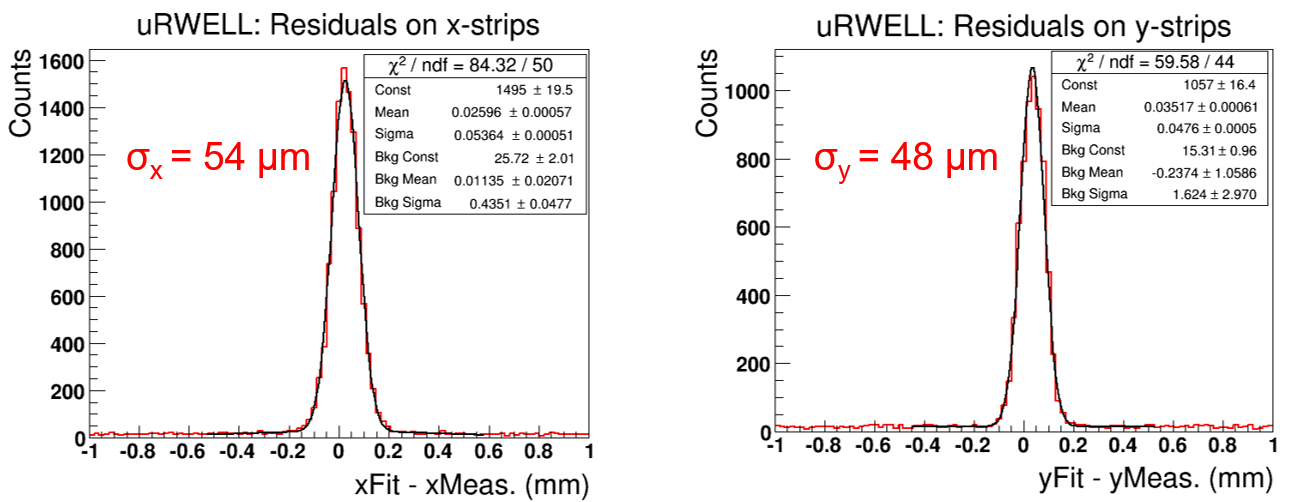
\includegraphics[width=1\columnwidth,trim={0pt 0mm 0pt 0mm},clip]{UVa_plots/uRwellResidual}
\caption{\label{fig:uRwellResidual} Residuals in x and y of the $\mu$RWELL prototype with the 120 GeV FTBF proton beam.}
\end{figure}
%
